
\chapter{Data analysis}

In this chapter our data sample will be analyzed according to the framework provided by Yoshikata Hatta. The angular correlation of jets is taken, and event mixing is used to factor out acceptance effects. 

[Something about the MC generation \cite{lheFormat}]


\begin{figure}[h!]
\begin{centering}
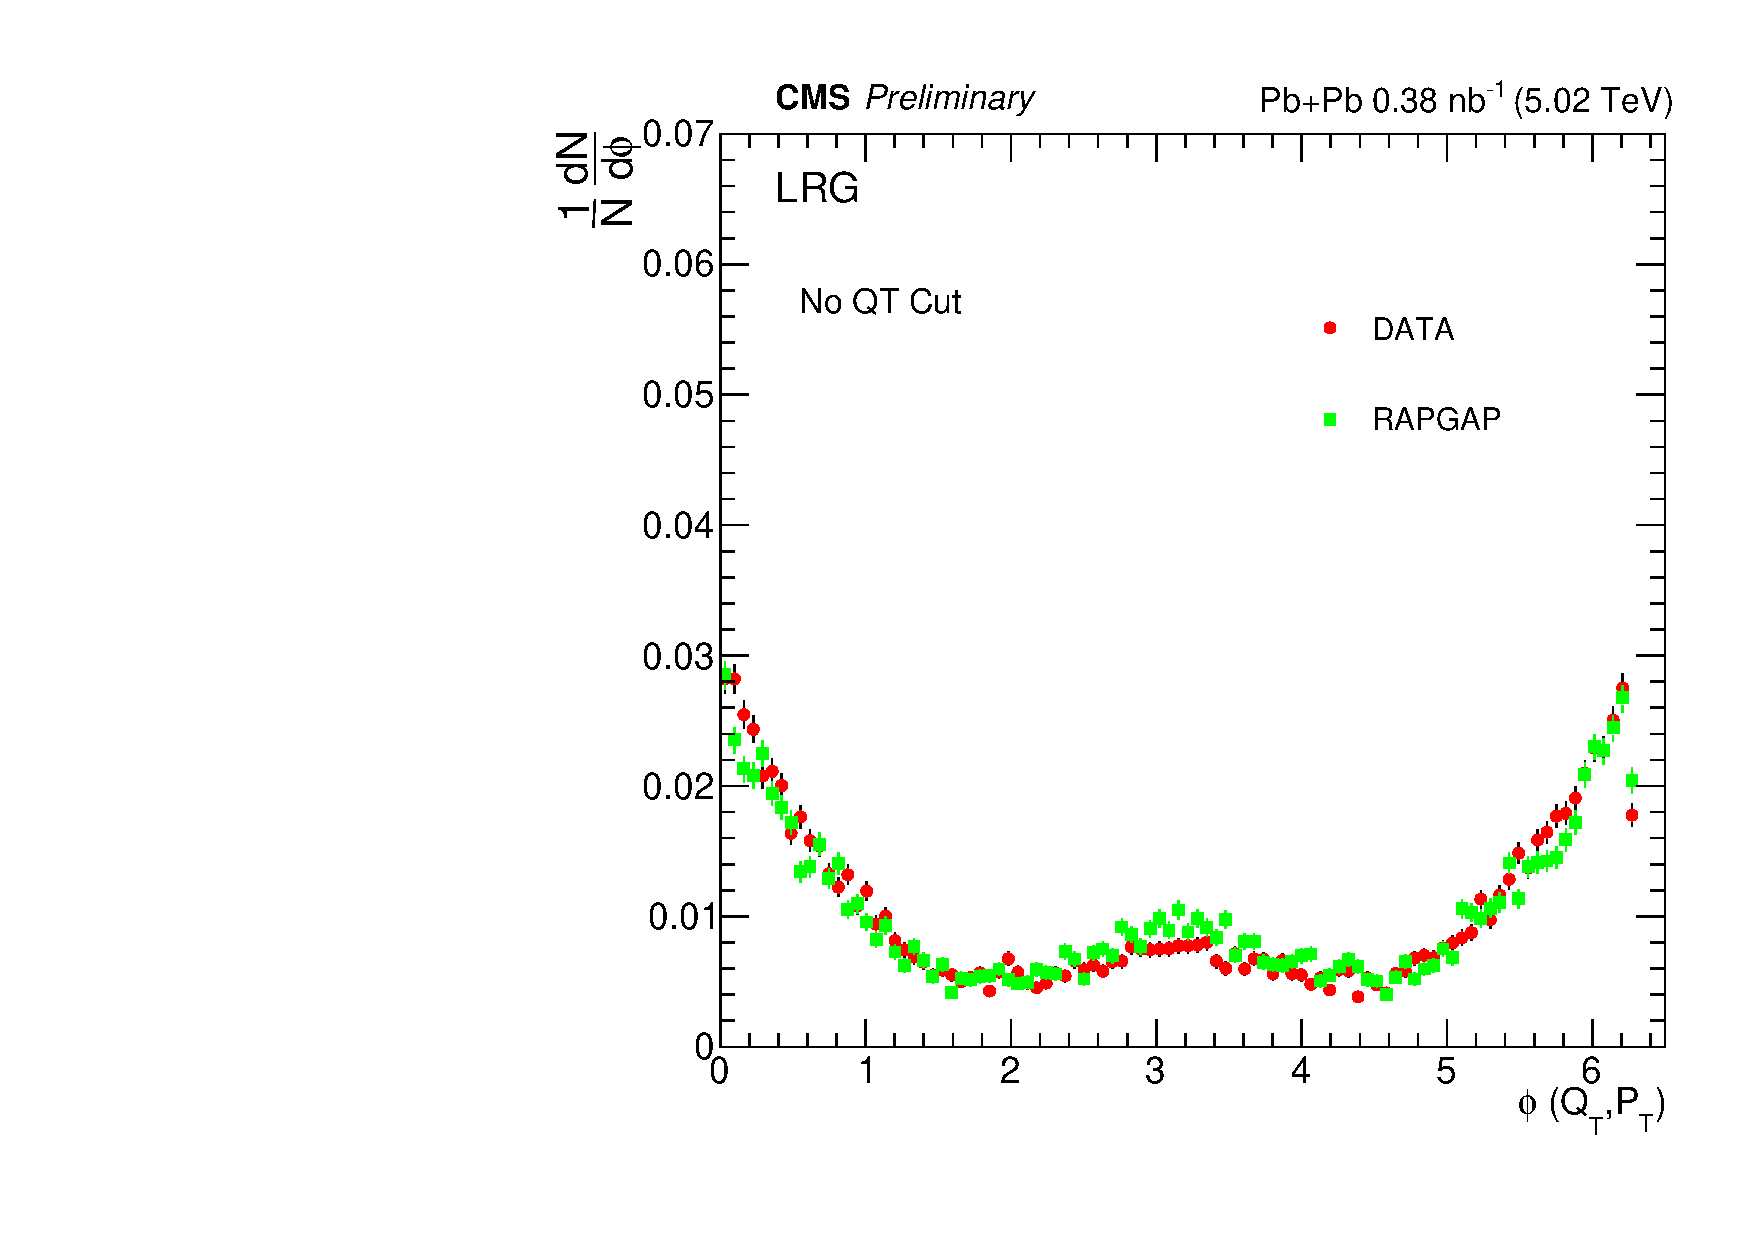
\includegraphics[width=6in]{Chapter6/importfigs/phi_allQt_raw.pdf}
\par\end{centering}
\caption{Raw $\phi$ distribution. \label{fig:rawPhi}}
\end{figure}

\begin{figure}[h!]
\begin{centering}
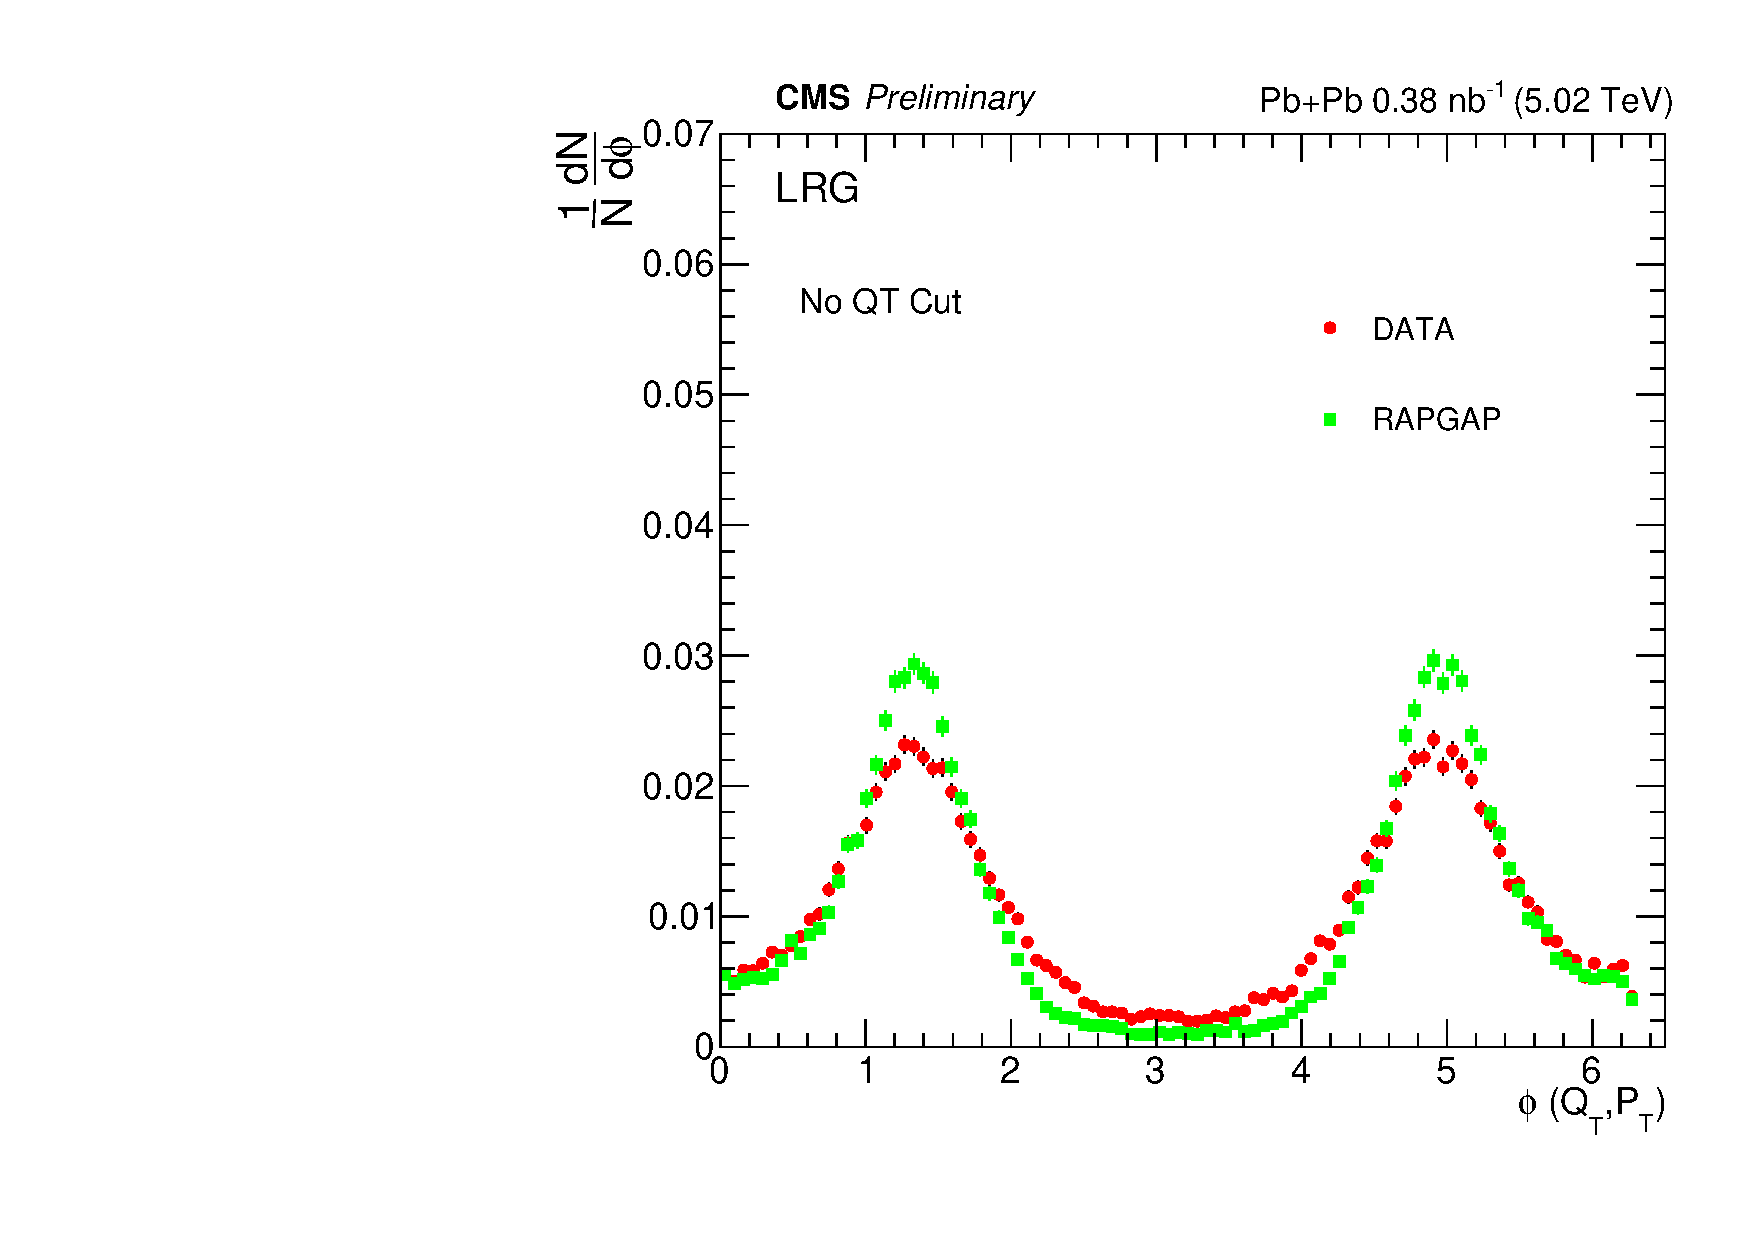
\includegraphics[width=6in]{Chapter6/importfigs/phi_allQt_mixed.pdf}
\par\end{centering}
\caption{Mixed $\phi$ distribution. \label{fig:mixPhi}}
\end{figure}

\begin{figure}[h!]
\begin{centering}
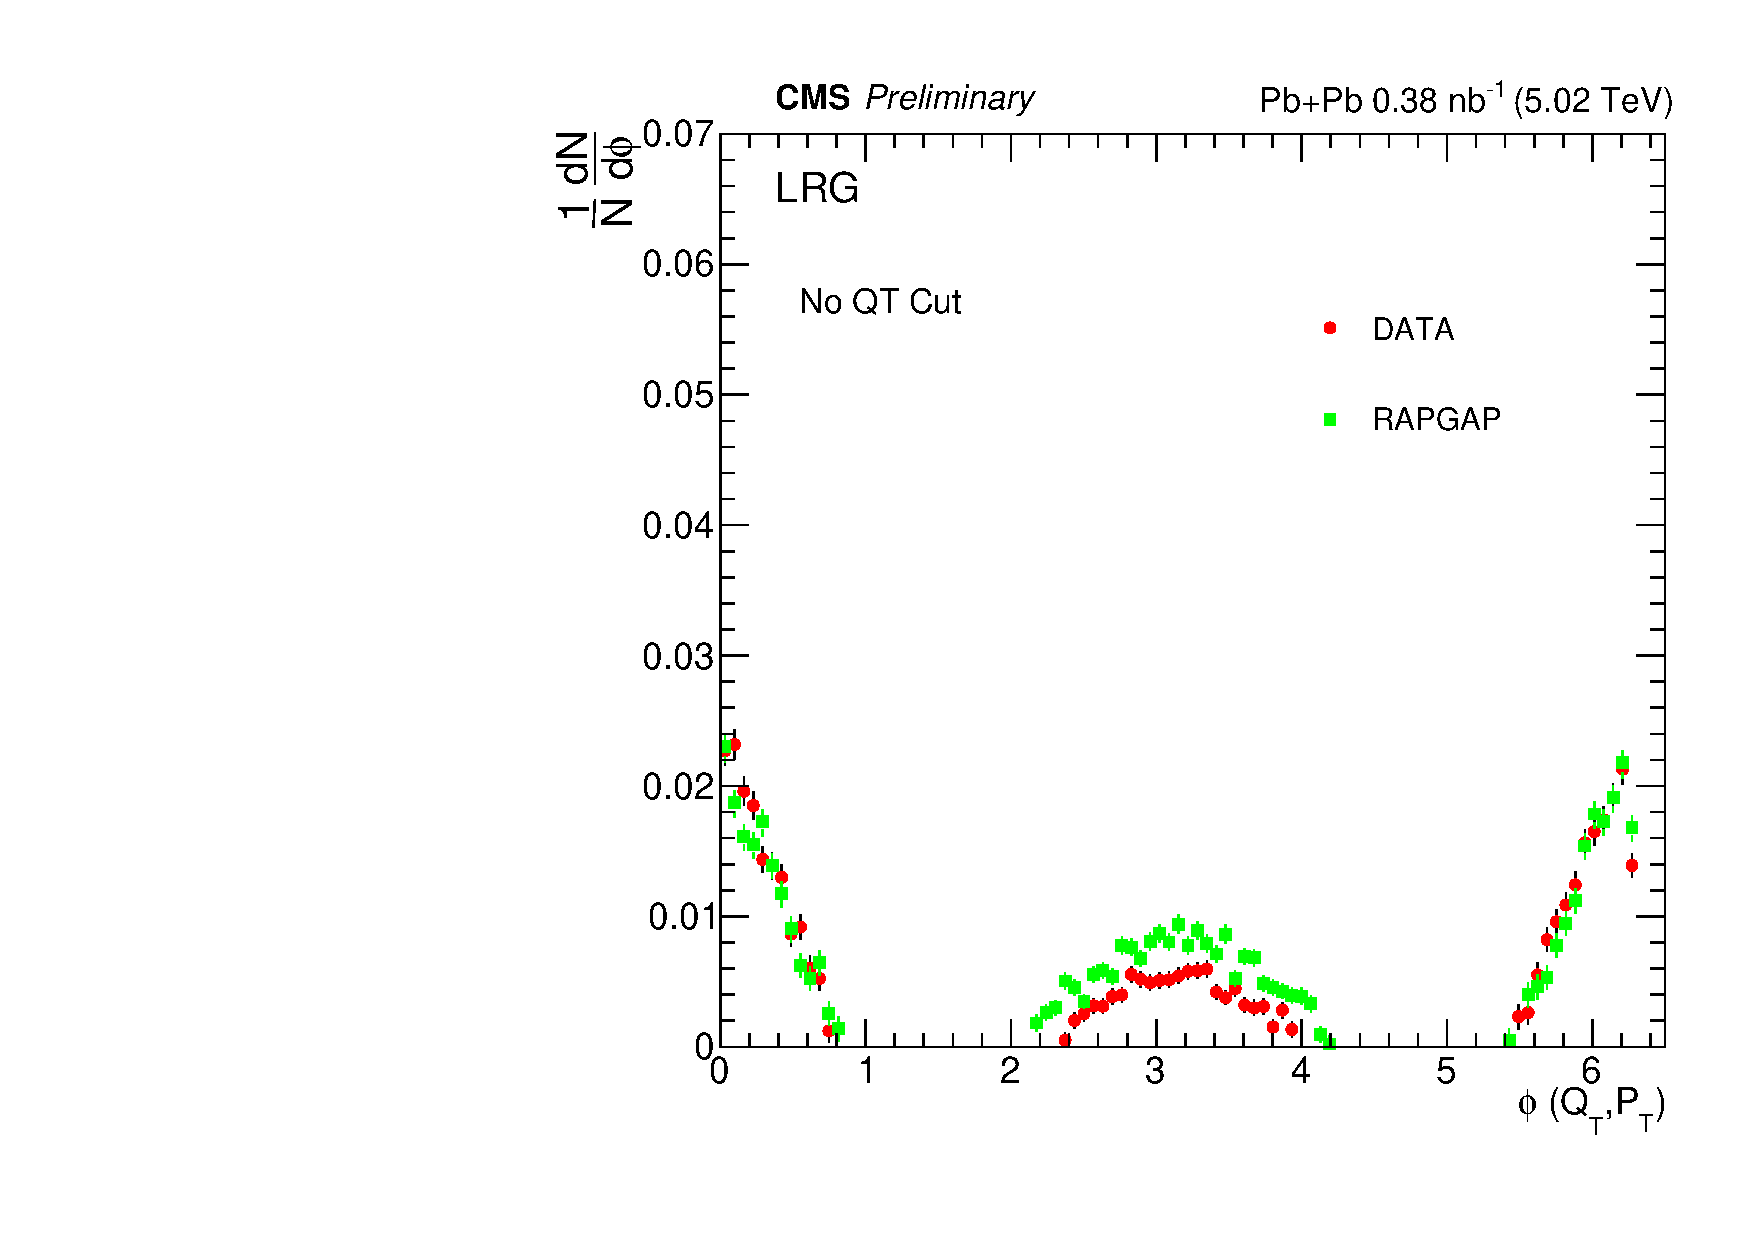
\includegraphics[width=6in]{Chapter6/importfigs/phi_allQt_subbed.pdf}
\par\end{centering}
\caption{Subtracted $\phi$ distribution. \label{fig:subPhi}}
\end{figure}

\begin{figure}[h!]
\begin{centering}
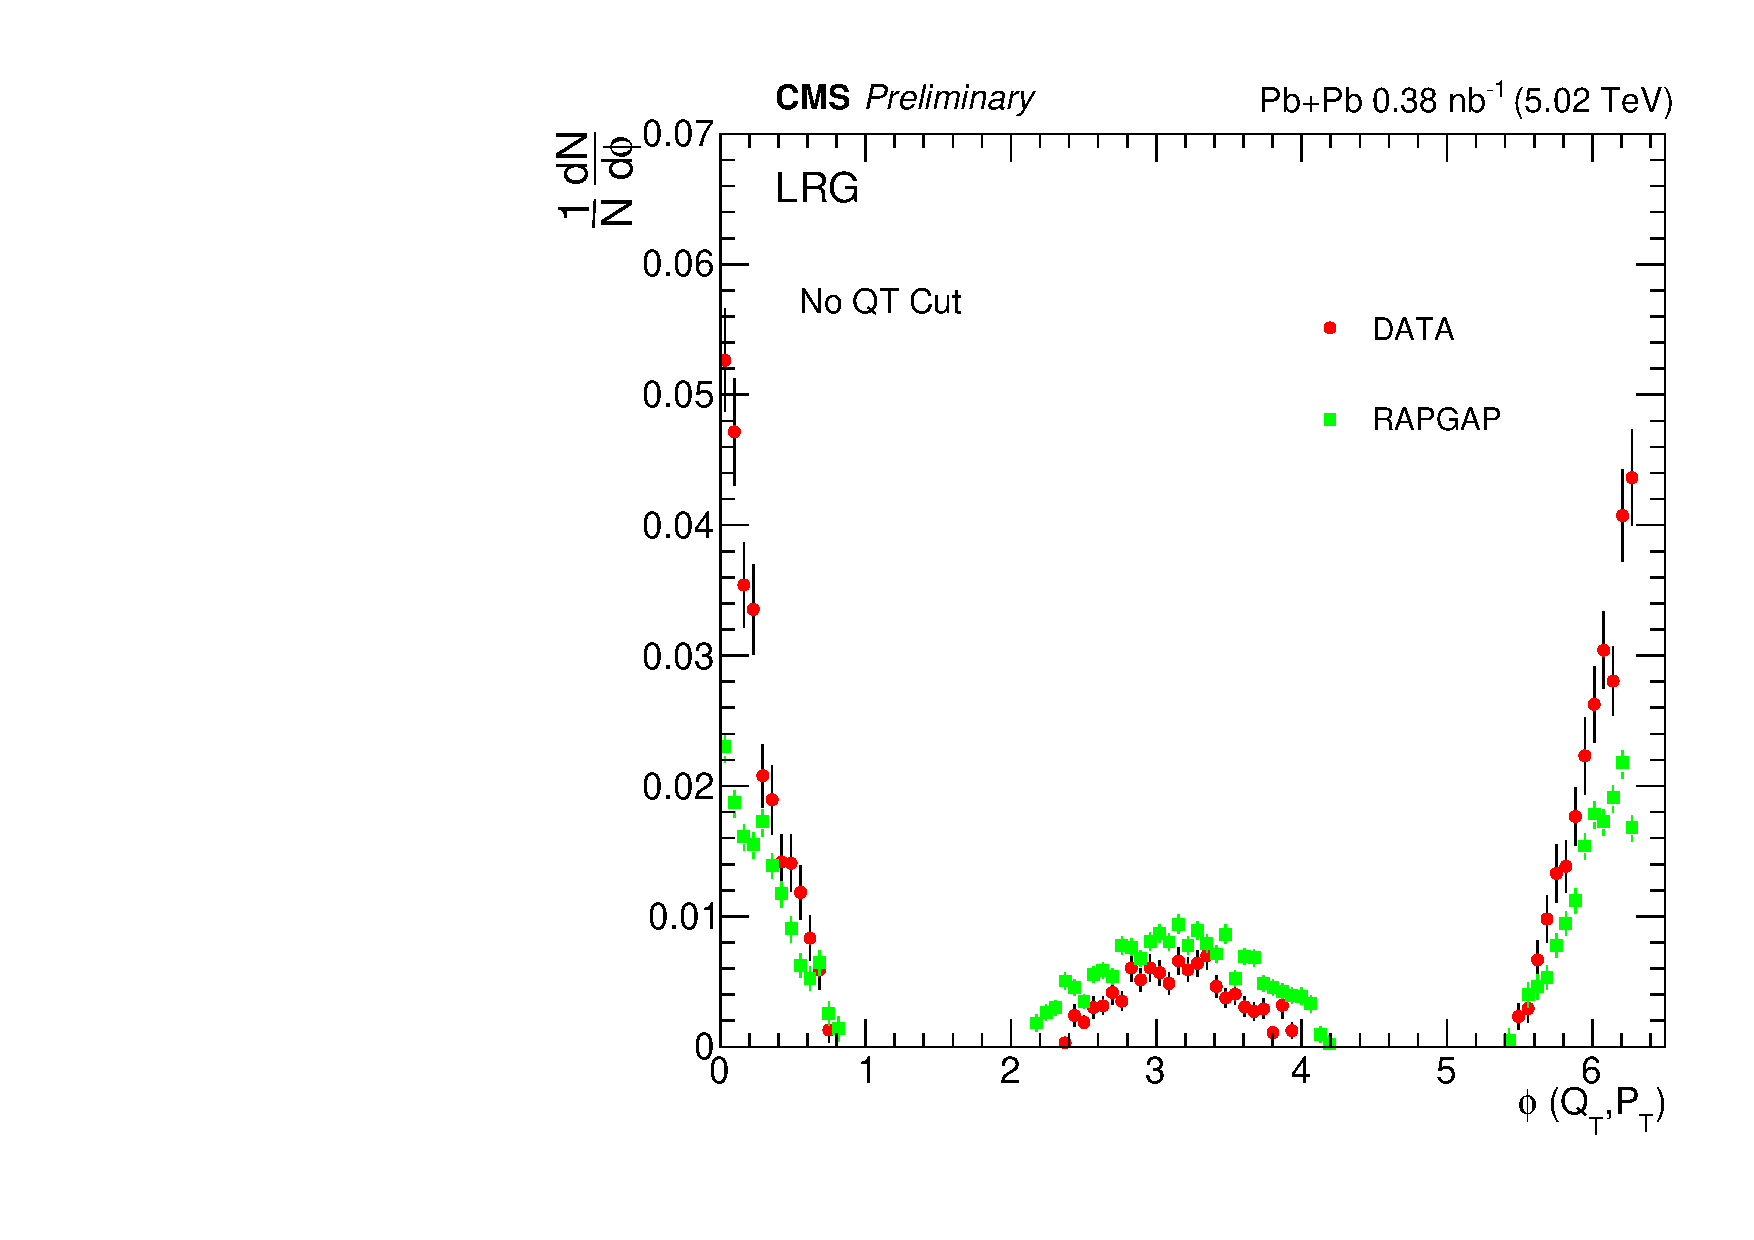
\includegraphics[width=6in]{Chapter6/importfigs/phi_allQt_final.pdf}
\par\end{centering}
\caption{Final $\phi$ distribution. \label{fig:finPhi}}
\end{figure}